\chapter{使用說明}

多年來研究室碩士班學生雖以\LaTeX 撰寫論文,文章結構多引用前屆學長論文結構,然共同的體裁檔一直欠缺,今從網路學習各校之體裁檔,加以正值著作期間,不斷瀏覽,收尋相關網頁,獲致許多相關知識,故解決多年困擾有望。此論文範本將{\tt ncuthesis}的使用說明以五章來陳述並做成中央大學標準論文格式,原始碼與PDF輸出皆放在''{\tt NCU}論文"的檔案夾內。請看{\tt README}說明於第三章內,其實只有三章重點,基於彰顯論文結構而將較不重要的小節亦以章的結構出現。
\begin{itemize}
\item {\color{red}紅色} ---  非常重要,因人而需修改。
\item {\color{blue}藍色} --- 必備知識,因需要而採用。
\end{itemize}
\index{ncuthesis 體裁!ncuthesisXe}\index{ncuthesis 體裁!ncuthesisCJK}
\section{文獻回顧}
此碩博士論文之體裁檔受啟發於兩位英美教授於網路上的公開文章與檔案
\begin{enumerate}
\item Class file: ociamthesis v2.2 (22/11/2010) \\
    By Keith A. Gillow $<$gillow@maths.ox.ac.uk$>$. \\
    Version 1.0 released 26/11/1997\\
	\url{http://www.maths.ox.ac.uk/help/faqs/latex/thesisclass}
\item "Minutes in less than Hours: Using \LaTeX\ Resources" \\
    by Jim Hefferon, $<$ftpmaint@tug.ctan.org$>$\\
	\url{http://tug.org/pracjourn/2005-4/hefferon/}
\end{enumerate}

\section{研究動機}
前述兩位教授的無私奉獻,進而激發自行學習撰寫體裁檔的願望。逢此畢業時節,最需要的體裁檔就屬符合中央大學碩博士論文的\LaTeX{}/\XeLaTeX{}體裁檔;在歐美國家,很多公、私立大學,都有屬於各校的檔案在網路上提供學生另一種選擇,讓研究生在低阻力,高效率下,輕鬆地做出字型美,排版佳,品質高,檔案小且全校統一的論文。然經網路搜尋後,中央大學無此資源與學生共享。心想,若撰寫成功則學生受惠,個人則增長知識且實驗室將有一致且符合校方要求的論文格式。

\section{研究目標}
撰寫體裁檔的目標是學生不需擔心論文設定問題。一切都由體裁檔負責。故其設計內容含 \par
\begin{table}[!hbt]
\centering             \index{\LaTeX!\textbackslash centering}
\caption{研究目標}
\begin{tabular}{cccccc}\\
論文封面 & 設定長寬 & 章節目錄 & 書脊文字 & 超連結 & 插頁技巧\\ 
編製頁碼 & 摘要附錄 & 字體行距 & 中文書籤 & 中文化 & 浮水印記\\
兩種編譯 & 多功選項 & 多種文書 & 程式撰寫 & 投影片\\
\end{tabular}
\end{table}

	準此,以上設定都以中央大學論文要求為準,至於其它大專院校論文格式\footnote{上網收尋並予此手冊比較。}應可自行修改,本手冊有提供修改方式及例題\footnote{其實97\%相同,不同在封面結構,摘要,與有無浮水印。},學生不須操心,認真閱讀、了解後自然會修改。
\section{中文化}
首先需中文化,此體裁檔採用國際上常用的兩種(亞洲字型,電腦內含字型)中文化結構:
\begin{itemize}
\item {\tt CJK (Chinese Janpanese Korean)}中文化: 使用pdf\LaTeX編譯。 
\begin{enumerate}
\item 使用{\tt titlesec, titletoc}處理章次及目錄。
\item 中文化相關巨集
{\tt CJKutf8,CJKvert,CJKnumb, fancyvrb},
{\tt verbatim, pdflscape, titlesec, titletoc} 已自動載入。不須再另行載入。
{\tt mypreamble.tex} 則提供其他讀者自訂巨集例如 
{\tt amssymb},{\tt amsmath,background,circuitikz}等,端視讀者需求。

\index{Packages!background}\index{Packages!tikzpicture}
\index{中文化!CJKutf8}\index{中文化!CJKvert}
\index{中文化!titletoc}\index{中文化!titlesec}
\index{中文化!CJKnumb}

\item 用 {\tt pdfLaTeX+MakeIndex+BibTeX}編譯。
\item 主檔案為{\tt masterthesis{\color{red}CJK.tex}及ncuthesis{\color{red}CJK}.cls}。
\end{enumerate}

\item {\tt xeCJK} 中文化: 使用\XeLaTeX編譯。\index{中文化!xeCJK}
\begin{enumerate}

\item 修改{\tt report class 內\textbackslash\char64chapter, \textbackslash\char64makechapterhead}處理章次及目錄。

\item 中文化相關巨集 
{\tt xltxtra,xunicode,CJKnumb,fancyvrb},
{\tt verbatim} 已自動載入。不須再另行載入。{\tt mypreamble.tex} 則提供其他讀者自訂巨集例如
{\tt amssymb,amsmath},{\tt background},
{\tt circuitikz}等,端視讀者需求。

\index{中文化!xltxtra}\index{中文化!xunicode}
\item 用{\tt XeLaTeX+MakeIndex+BibTeX}編譯。
\item 主檔案為{\tt masterthesis{\color{red}Xe.tex}及ncuthesis{\color{red}Xe}.cls}。
\end{enumerate}
兩種主檔案兩者不同之處其實只有10行左右。但為方便不同的研究生使用,故刻意做出兩份。雖然台灣有其他 $\chi$\TeX({\tt aka. chi\TeX}),cw\TeX,PU\TeX的相同軟體,但編譯時可能有兩種中文相衝的可能性,未深入研究。
\end{itemize}

\section{論文結構}
稍微了解\TeX{}/\LaTeX\ 的學生讀者應可了解下列結構,因為是沿用\LaTeX\ {\tt report}結構。只是體裁檔{\tt (class file)}需寫入{\tt ncuthesisCJK}\hfil\break或{\tt ncuthesisXe}以便做出符合中央大學範例的格式。%
\index{\LaTeX!classes!report}\index{\LaTeX!classes!article}
\index{\LaTeX!\textbackslash chapter}\index{\LaTeX!\textbackslash section}\index{\LaTeX!\textbackslash subsection}\index{\LaTeX!\textbackslash subsubsection}\index{\LaTeX!\textbackslash author}\index{\LaTeX環境!table} \index{論文結構}
\label{bookstruc} \index{\LaTeX!\textbackslash label}
\begin{table}[hbt!]
\caption{論文結構}
\end{table}
\fvset{frame=topline,numbers=left,numbersep=3pt,
firstline=1,lastline=1}
\VerbatimInput{masterthesisXe.tex}
宣告區\quad {\tt Preamble}
\fvset{frame=topline,numbers=left,numbersep=3pt,
firstline=22,lastline=22}
\VerbatimInput{masterthesisXe.tex}
本文區\quad {\tt Text body}
\fvset{frame=bottomline,numbers=left,numbersep=3pt,
firstline=52,lastline=52}
\VerbatimInput{masterthesisXe.tex}

\index{\LaTeX!\textbackslash VerbatimInput}
此資料夾提供兩種中文化方法,使用時先選擇主檔(建議\XeLaTeX\ 編譯方式),然後將{\tt masterthesisCJK.tex} 或 {\tt masterthesisXe.tex} 另存新檔,給一個自己喜歡的檔名譬如{\tt foo.tex}。新檔內容幾乎一模一樣不需改變甚麼(所以簡單吧)。但是至少系所、學生、教授、論文題目不同,須修正,現將分別陳述於後: \index{\LaTeX!\textbackslash input}
\index{Packages!verbatim}\index{foo}

\subsection{宣告區}

\fvset{frame=single,numbers=left,numbersep=3pt,
firstline=2,lastline=5}
\VerbatimInput{masterthesisXe.tex} 
\index{\LaTeX!\textbackslash VerbatimInput}
宣告區內2-3行是本檔使用的外來巨集(必要具集則在{\tt*.cls}內)。
\fvset{frame=single,framerule=1mm,numbers=left,numbersep=3pt,
rulecolor=\color{red},firstline=6,lastline=16}
\VerbatimInput{masterthesisXe.tex} 
6-16行是系所、學位、論文題目\footnote{亦可填入非學位性的研究計畫,讀書計畫等。}、研究生、指導教授可照論文範例填入相關資訊。共同指導教授(預設是無)亦可填二位。\index{宣告區}
\index{ncuthesis 指令!\textbackslash mprof} \index{ncuthesis 指令!\textbackslash sprof} \index{ncuthesis 指令!\textbackslash sprofa}
\index{ncuthesis 指令!\textbackslash title} \index{ncuthesis 指令!\textbackslash subtitle}\index{ncuthesis 指令!\textbackslash degree} \index{ncuthesis 指令!\textbackslash degreedate}\index{ncuthesis 指令!\textbackslash author}
\index{ncuthesis 指令!\textbackslash copyyear}\index{ncuthesis 指令!\textbackslash dept}%
\fvset{frame=single,framerule=0.4pt,numbers=left,numbersep=3pt,
rulecolor=\color{black},firstline=17,lastline=21}
\VerbatimInput{masterthesisXe.tex} 
17行是自行定義的中文化定理、引理、例題等具重複性常用定義。
如果自訂巨集少則自行加入,若多則建議寫入{\tt mypreamble.tex},再以\textbackslash {\tt input}引入。如範例所示。 第21行則是要求索引製作。
\index{ncuthesis 檔案!mypreamble}\index{ncuthesis 檔案!ncuthesisCJK}\index{ncuthesis 檔案!ncuthesisXe}\index{ncuthesis 檔案!abstractcn}\index{ncuthesis 檔案!abstracten}
\index{ncuthesis 檔案!chapter1}\index{ncuthesis 檔案!chapter2}\index{ncuthesis 檔案!appendA}\index{ncuthesis 檔案!appendB}\index{ncuthesis 檔案!bibli}\index{ncuthesis 檔案!symbol}\index{ncuthesis 檔案!acknowledge}
\index{Packages!calculator}\index{Packages!showframe}
\index{Packages!hyperref}\index{Packages!fancyvrb}

\subsection{本文區}
\fvset{frame=single,numbers=left,numbersep=3pt,firstline=23,lastline=32}
\VerbatimInput{masterthesisXe.tex}
這些行是製作封面,書名頁,非\LaTeX{}格式但已成為PDF格式紙張插頁,例如各校口試委員簽名頁等畢業有關之頁。

\fvset{frame=single,framerule=1mm,numbers=left,numbersep=3pt,
rulecolor=\color{blue},firstline=33,lastline=39}
\VerbatimInput{masterthesisXe.tex}
35-39行依序為中英文摘要、謝誌、目錄、圖目、表目、符號說明等。 因論文需要而設計的特定環境(不需要則不必寫,用\%使其\textbackslash include指令無效)。\index{\LaTeX環境!tabbing}

\index{ncuthesis 環境!abstractcn} \index{ncuthesis 環境!abstracten}\index{ncuthesis 環境!acknowledgements} 
\index{ncuthesis 環境!symbols}\index{ncuthesis 環境!appendA}\index{ncuthesis 環境!appendB}

\fvset{frame=single, framerule=1mm,numbers=left,numbersep=3pt,
rulecolor=\color{blue},firstline=40,lastline=48}

\VerbatimInput{masterthesisXe.tex}
第43-48行用\verb|\include|加入其他各章節,是屬\LaTeX的用法,如同打字一般,將文字內容打入各檔案。第二章有簡要說明\LaTeX用法。
48行是參考文獻設定。本書用簡單的方式,另有檔案方式({\tt.bib}),請看第二章。

\fvset{frame=single,framerule=0.4pt,numbers=left,numbersep=3pt,
rulecolor=\color{black},firstline=49,lastline=51}
\VerbatimInput{masterthesisXe.tex}
49-51行是為了了解紙張設定,可除去(\%)不用。

\subsection{插頁}
本論文封面已設計成中大碩博士論文封面,然因中央大學有其它表格化的{\tt doc}檔,此手冊並未以\LaTeX設計其相關表格,以維持與其他學校論文架構最大的相容性,方便推廣至其他大專院校。然如何加入特定表格?建議用插頁方式如下。先完成{\tt DOC}相關表格\todo[inline]{此表格學生需自行確認是最新版},排好順序,再存成{\tt myfile.pdf}檔,其中每一頁之後皆要插入空白頁,才能保證出現在奇數頁。所以若有非\LaTeX的{\tt pdf}檔皆可以類推,加入論文內。
\index{ncuthesis 檔案!committee}
\begin{verbatim}
1. \usepackage{pdfpages}    % 於宣告區
2. 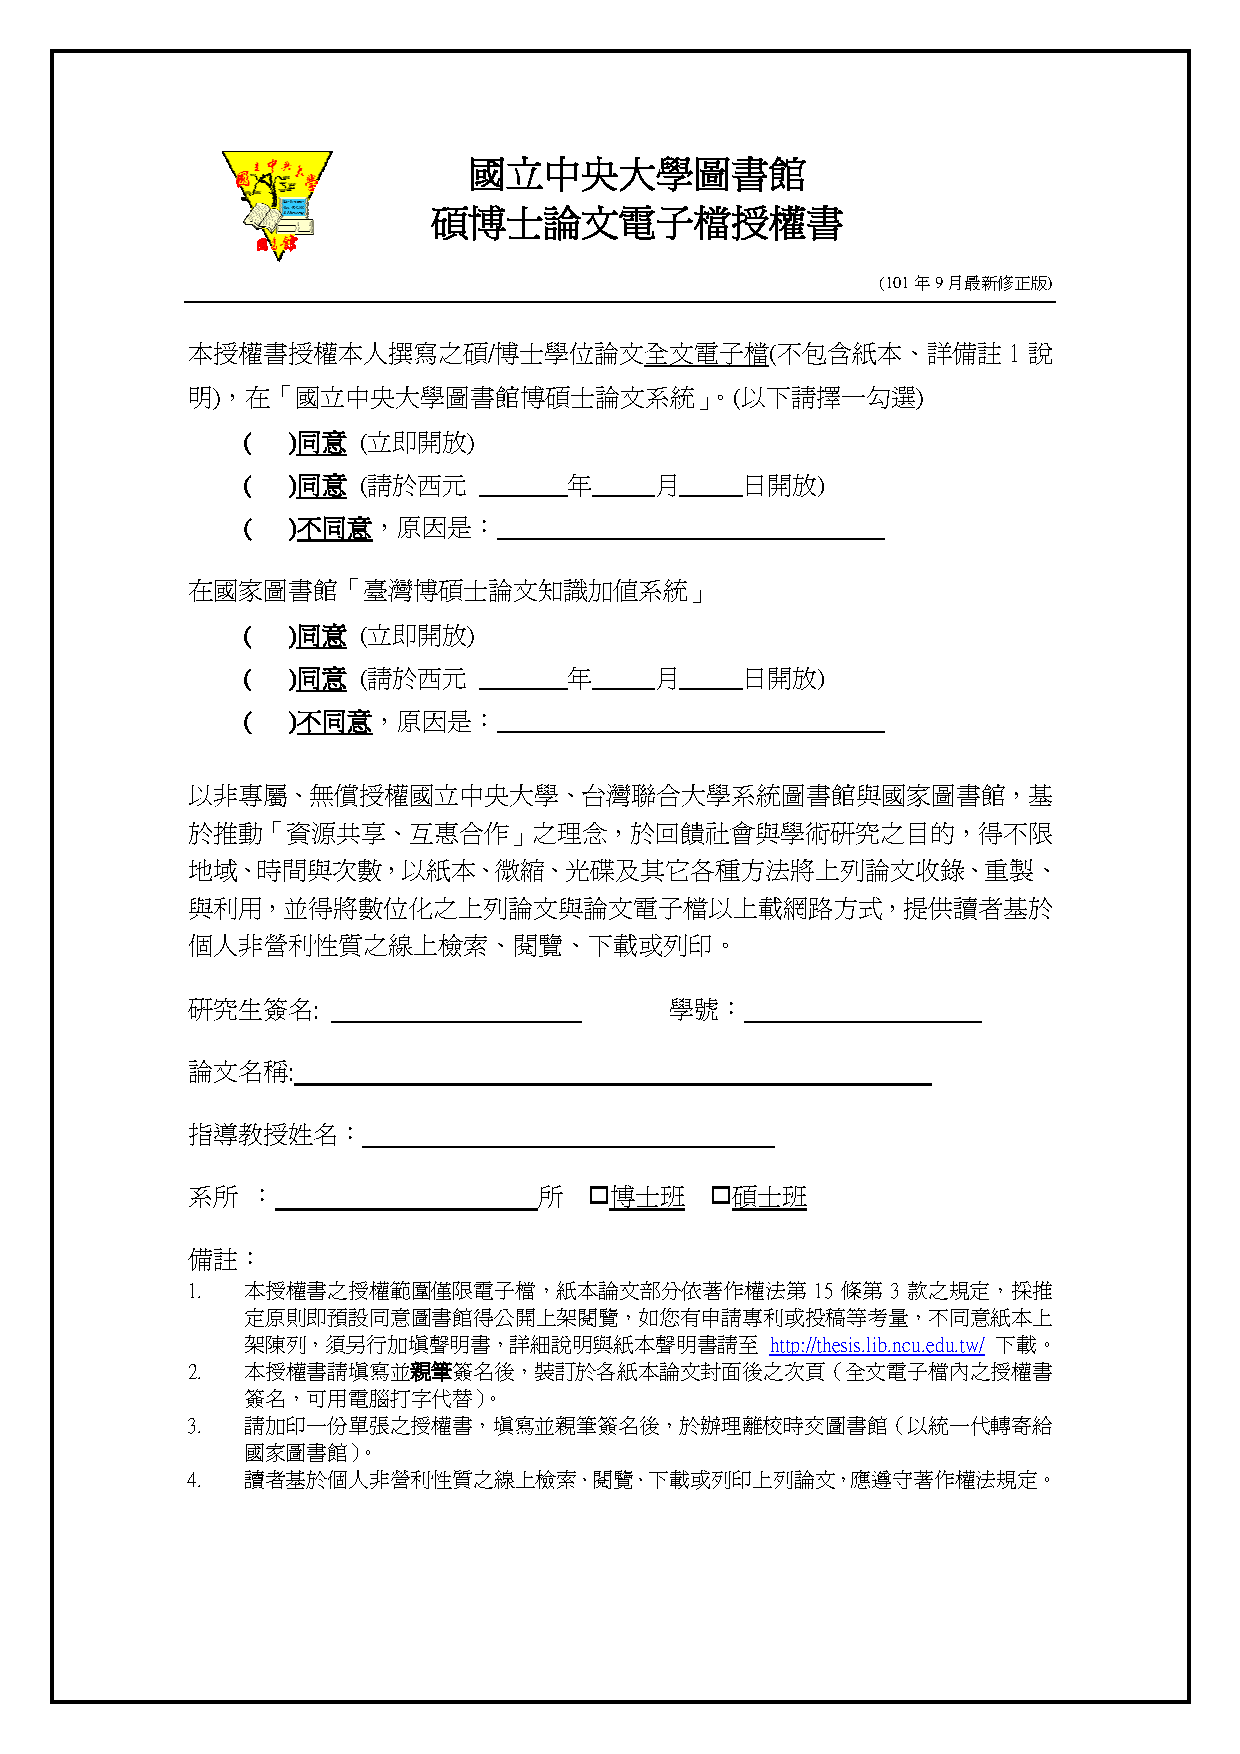
\includepdf[pages=-,     % - =所有頁面 或用 1,2 表示
      addtotoc={1,subsection,2,{書簽名},標名}]{myfile.pdf}
註解:addtotoc={page number,section,level,heading,label}
\end{verbatim}

第1行寫於宣告區。插頁若需出現在目錄則加{\tt addtotoc}指令。上述之第2行於插頁需要之處寫入。如本例第32行所示,再次顯示於下:
\fvset{frame=single,framerule=1mm,numbers=left,numbersep=3pt,
rulecolor=\color{blue},firstline=32,lastline=32}
\VerbatimInput{masterthesisXe.tex}

另外有些博士生將履歷 ({\tt via package moderncv}) 加入論文最後幾頁,亦可用此技巧達成。所以只要是非以\LaTeX產生的圖表轉成{\tt png,jpg,jpeg,pdf}檔後,皆可依此方式加入論文並與論文成為一體自動連號。

\section{結語}
簡而言之,此論文的主檔案有兩類
\begin{itemize}
\item {\tt masterthesisCJK.tex} 及必需之體裁檔 {\tt ncuthesisCJK.cls}
\item {\tt masterthesisXe.tex } 及必需之體裁檔 {\tt ncuthesisXe.cls}
\end{itemize}
提供論文編寫方式,其輸出即是標準格式。快速、方便、及時。
\index{\LaTeX環境!itemize}
\begin{itemize} \index{\TeX!\LaTeX}
\item 本論文假設學生有 \TeX/\LaTeX 基礎知識,若需加強相關知識,網路上有免費資訊可供學習。第二章亦提供一些入門知識及參考網址。 \index{使用手冊}

\item 第20行:可只編譯某些檔(以逗點分開),除錯時好用,可降低編譯時間。
\fvset{frame=single,numbers=left,numbersep=3pt,
rulecolor=\color{blue},firstline=20,lastline=20}
\VerbatimInput{masterthesisXe.tex}

\item 第25行:中文字大小及行距是由這行設定
\fvset{frame=single,numbers=left,numbersep=3pt,
rulecolor=\color{blue},firstline=25,lastline=25}

\VerbatimInput{masterthesisXe.tex}

\item 使用亞洲字型{\tt CJK,xeCJK}中文化且設定為楷書({\tt bkai}),不是 cw\TeX 或 PU\TeX 或 $\chi$\TeX。 \index{\TeX!cw\TeX}\index{\TeX!PU\TeX}

\item 使用時需有{\tt unicode/utf8}編輯器如{\tt MiKTeX的TeXworks}\footnote{LyX愛好者可先將檔案({\tt chapter1,2,3...})做好再存成{\tt .tex}檔然後用{\tt masterthesis.tex}編譯}。 \index{MiKTeX}\index{TeXworks} \index{\TeX!LyX}\index{\TeX!\XeLaTeX}

\item {\color{red}行動安裝}在第二章說明,{\tt Window/Android}版免費排版系統\linebreak \TeX{}/\LaTeX{}/\XeLaTeX{}垂手可得,亦建議採用。 

\item 使用pdf\LaTeX或 \XeLaTeX連續編譯兩次({\tt TeXworks} 會自動執行兩次)。故若有圖檔請都存成{\tt png, jpg, jpeg, pdf}。

\item 撰寫方式如\TeX/\LaTeX{}一般寫作技巧。此範例主要是用環境\linebreak({\tt environment}) 技巧。除"\,附錄"環境外,所有其他環境皆會自動帶入論文題目。\label{indpage}

\item {\color{red}論文很少用索引,故{\tt makeidx,\textbackslash makeindex,\textbackslash printindex}三指令(第2、34行,最後一行在{\tt bibli}內) 可省略,但此論文範本保留,以便保有科技書籍的格式,請看第\framebox{\pageref{others}}頁。}

\item {\tt bookbone.tex}提供製作論文書脊,現印於右側以便觀察 (\XeLaTeX{}則無法呈現!?) 
長書脊時請仿照校名({\tt tabular}技巧)製作兩欄式,只要單獨編譯{\tt bookbone.tex} 即可得。 \index{ncuthesis 指令!\textbackslash backbone}
%\marginpar[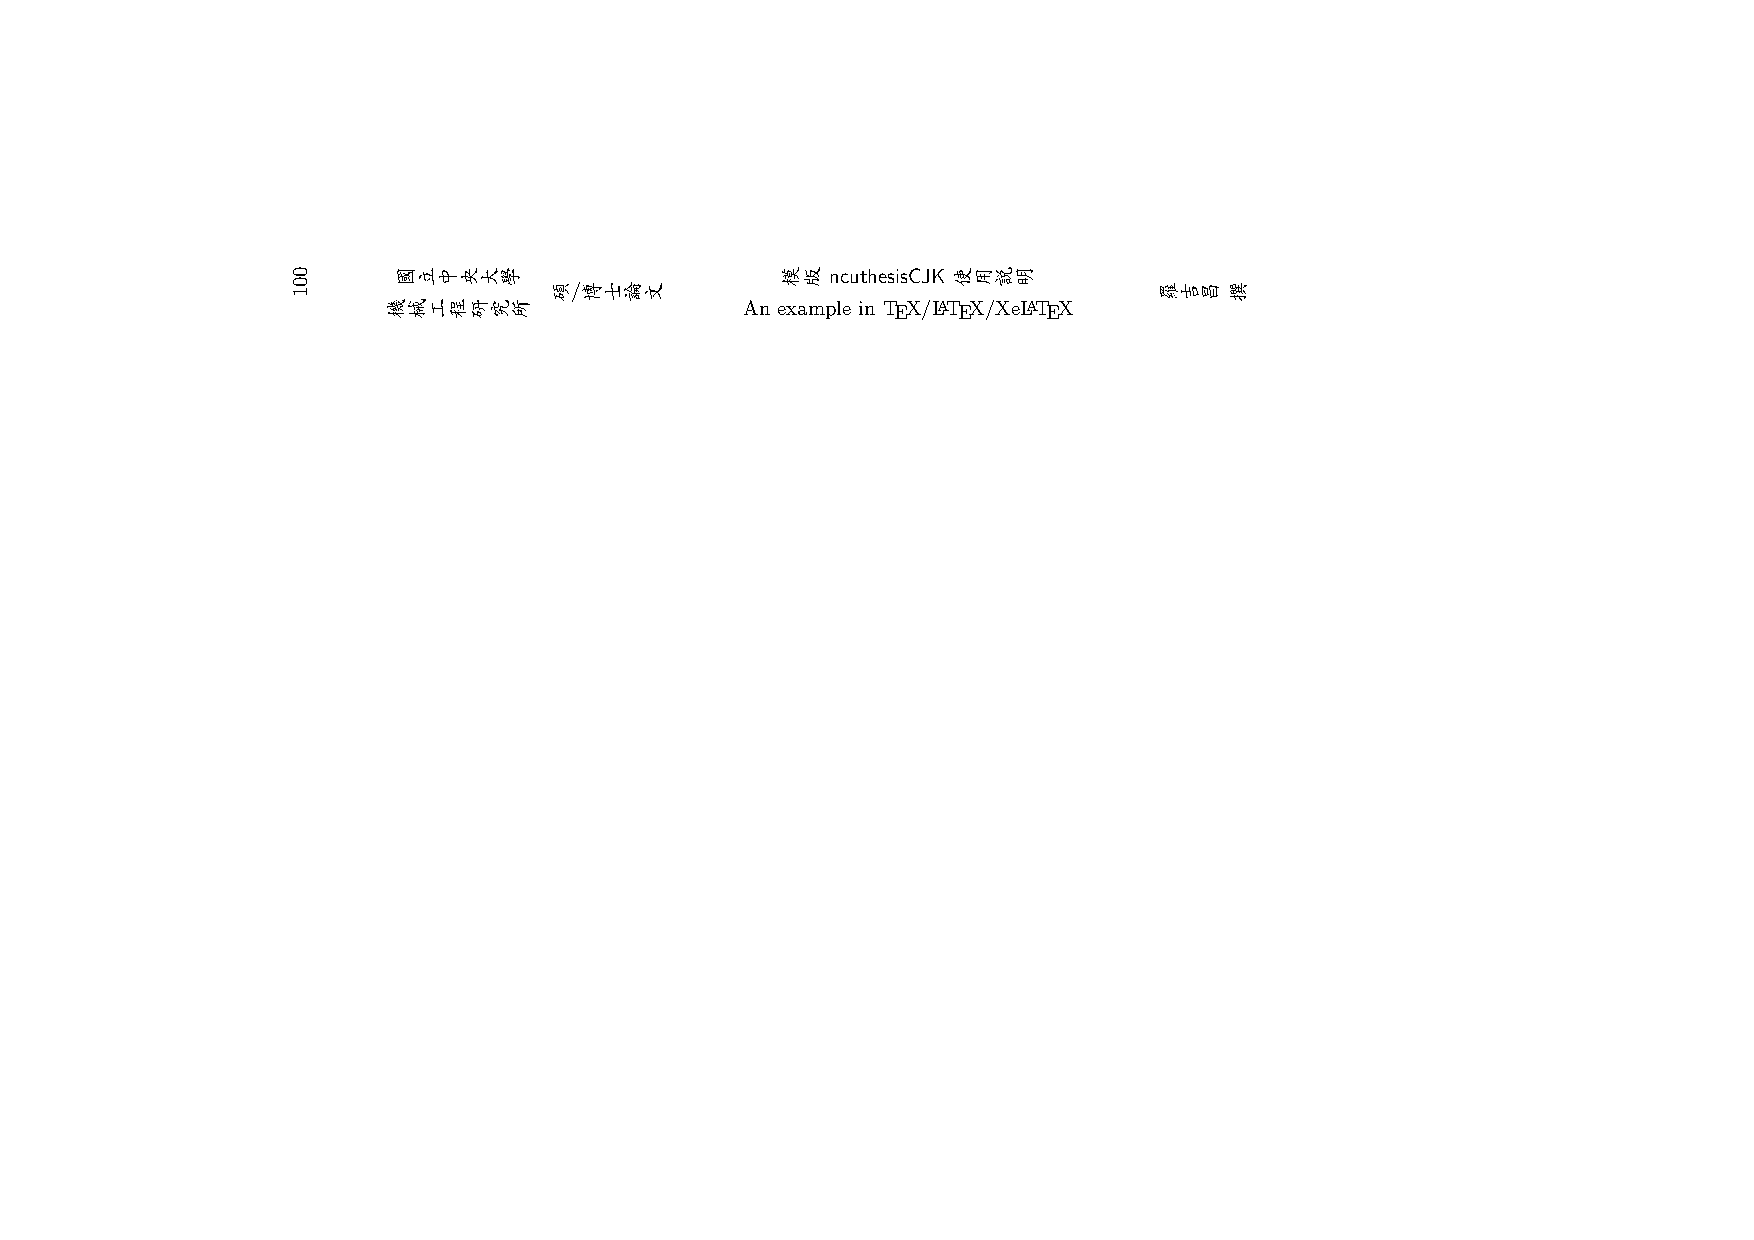
\includegraphics{bookbone.pdf]{}

\item 本論文用到的輸入參數整理在符號說明頁。了解後就可開始用此套件了。\label{conclude}

\item 編譯時,可選單面印刷(預設值)或雙面印刷: \index{\LaTeX!\textbackslash noframe}%
單面印刷({\tt oneside}) -- 適合一般計畫({\tt project})或報告({\tt report})。\\
雙面印刷({\tt twoside}) -- 適合正式文件({\tt thesis}),有封面,謝誌等。
\item 另外有四種工作模式可選擇:\\ \index{\LaTeX!\textbackslash draft}
\index{\LaTeX!\textbackslash marginnote} \index{\LaTeX!\textbackslash raggedright} 
\index{\LaTeX!\textbackslash raggedleft}
{\color{blue}
\begin{center}
\begin{tabular}{|c|c|c|} \hline 
 選項          &  空白    &  {\tt  draft}      \\ \hline 
 空白          &    框    &    框 +頁眉      \\ \hline
{\tt noframe}  &    無框  &    無框+頁眉   \\ \hline
\end{tabular}
\end{center}
}
空白是單頁印刷({\tt oneside}),因為是預設值。若改為{\tt twoside}則為雙頁印刷,故單面印刷有四種,雙面印刷又重複四種。

\begin{enumerate}
\item $<$空白,空白$>$此預設值會產生文字外框,偵測是否越界。
\item $<${\tt draft},空白$>$選項,編譯較快,圖形或插頁皆以方格表示並不載入,且右邊會出現黑體垂線表示超出頁面範圍,方便修改除錯。且頁眉右側會出現智財權屬於作者,以防止文件不慎遺出。
\item$<$空白,{\tt noframe}$>$除去外框之{\color{red}單頁印刷完稿},要雙頁印刷之完稿,別忘了要用{\tt twoside}{\color{red}。的確,$<${\tt twoside,noframe}$>$才是最後完稿。}\todo[inline]{切記!切記! [disable] for removing todos, [twosides, noframe] for final version。}但有些學校論文少於100頁可採單頁印刷。


\item$<${\tt draft,noframe}$>$無外框但有頁眉。
\end{enumerate}
\item \textbackslash printpapersize 會印出目前頁面參數。
{\tt ncuthesisXe.cls}檔案內第51-57行(請參看附錄一),可改變紙張大小。\\
\framebox{
\printpagesize 
}\\               % to print page size
上示參數為相對於紙張左上角(視為原點),向右向下(1in,-1in)處之參考點。\index{ncuthesis 指令!\textbackslash printpapersize}
\item \LaTeX有五種體裁檔{\tt article, book, report, letter, slides}\hfil\break{\tt ncuthesisXe(CJK)}則是結合{\tt report}再定義新環境而成。故要產生本校的固定格式必需用{\tt ncuthesisXe(CJK)}。\index{\LaTeX!\textbackslash hfil}
\index{\LaTeX!classes!article}\index{\LaTeX!classes!book}\index{\LaTeX!classes!report}
\index{\LaTeX!classes!letter}\index{\LaTeX!classes!slides}
\item 浮水印的程式碼在{\tt mypreamble.tex}內,需{\tt background}套件(手冊);不需要者可用(\%)除去。中央大學不需浮水印,但設計它的原因是(1)可放大改成時間或加入防拷貝字語,(2)可置於頁面任何位置(包含斜放),(3)其他學校(清大,台科大,北科大)有浮水印需求。\index{watermark}\index{浮水印}
\item 論文寫作的過程中,常常需要自我提醒,要修改這,修改那,要加入圖表等代辦事項。這時我們可用\verb|\todo[inline]{提醒內容}|\todo[inline]{提醒內容}立即於寫作的同時加入,它會以橘色顯示在論文中以免忘記。這些提醒事項都會收錄在單頁{\tt List of todos}中,一目了然,非常好用。當然完稿時,切記要以{\tt \textbackslash usepackage[disable]\{todonotes\}}除去所有提醒、代辦事項;不然你的論文有很多代辦事項卻是正式文件。
\end{itemize}

\section{其他文書\label{others}}\index{其它文書}

此一節是為了想了解如何修改程式碼的讀者而寫的,尤其是非中央大學的研究生。例如 (1)某大學的研究生也想使用此套件來寫論文,但中央格式與該校不同;(2) 某研究生想為該校寫出適合該校的\LaTeX碩博士論文套件,並發表於網路上且會維護它; (3) 想進一步學習\LaTeX基礎者,則須研究本節。所以不是這目的的讀者可跳過這一節。

此檔案夾可製作的文書不止論文而已,其實只要稍微增修就可產生很多其他文書結構。各行各業中常見的文書有

\begin{itemize}
\item 書 --- 封面、摘要、章節、附錄、索引、文獻。

以論文首頁做為書的封面較罕見,大部分需牽涉封面設計,故此頁需請專人設計。其實\LaTeX的封面設計({\tt book design})可自己設計,需上網學。

\item 論文 --- 首頁、摘要、章節、附錄、文獻。

這是此手冊的主要目標。其它大專院校論文格式需自行更改,其實論文主體(目錄、章節、附錄、索引、文獻) 因教育部法規已定,各校一致性頗高,剩下的約十頁左右,有明顯差異(例如中英文摘要多了姓名及系所)。故根據下列方向修改,各校論文99\%的吻合度是可達成的。
\begin{itemize}
\item 封面格式:{\tt ncuthesis.cls}檔,約在{\tt 167-202}行。
\begin{itemize}
\item [1] 熟悉\LaTeX者可直接修改。\index{\LaTeX!\textbackslash titlepage}
\item [2]  自動化  以{\tt \textbackslash (re)newcommand}定義指令{\tt \textbackslash commands},請參考附錄二。

\item [3] 手動化 用{\tt titlepage}環境撰寫,請參考附錄二。

\item [4] 以{\tt doc}製作封面後轉成{\tt pdf}以取代中央封面,此法最快,但\LaTeX均質性較差。其實{\tt myfile.pdf}的目的即是為此而設計。
\end{itemize}
\item 中英文摘要:亦可類推。這部分是各校差異所在。附錄二亦有用\verb|\renewenvironment{onecol}|修改,可參考附錄二。

\item 紙張大小:都是{\tt A4}紙張,但內文四周留白寬度可能稍微不同,這可由{\tt ncuthesis.cls}檔內修改,約在{\tt 51-57}行。
\item 字體索引:詳見第\fbox{\pageref{indpage}}頁。
\item 去浮水印:{\tt mypreamble.tex}內,刪除相關指令。
\item 章節標題:本校用中文數字一、二、三為章次編號,有些學校則用第一章,第一節來編號,欲改為後者可將{\tt ncuthesis.cls}內第{\tt 85}行加入兩中文字,改\verb|\CJKnumber{\arabic{chapter}}、|改為
{\color{red}第}\verb|\CJKnumber{\arabic{chapter}}|{\color{red}章},餘類推。
\item 增加目錄:若要將"\,論文審定書"加入目錄,則加入下列兩行於審定書之前即可,餘類推。
\begin{verbatim}
\cleardoublepage\phantomsection     % 強制奇數頁開始
\addcontentsline{toc}{chapter}{論文審定書}% 加入目錄
其中 chapter 亦可改為 (sub/sub)section.
\end{verbatim}
\end{itemize}

\item 報告(論文計劃書) --- 首頁、摘要、章節、附錄、文獻。

報告稍微正式,故封面可沿用論文封面。

\item 作業 --- 首頁、章節。\index{其它文書!作業}

首頁 改寫 姓名、學號、班級、科目,如果希望不要單獨一張封面(因較非正式或浪費),請參考附錄二。


\item 會議記錄

如作業範例所示,稍微修改上半部的內容及將"\,作業環境"改為"\,議題環境"即可。要更正式一點,請看文獻回顧第二篇
。\framebox{Back\pageref{conclude}}
\end{itemize}

\section{編譯失敗}
目前,此體裁檔在六台不同的電腦(皆{\tt Windows})及一台{\tt Ubuntu上安裝LyX2.0.2/TeXLive2009},測試成功,都是安裝英文\LaTeX{},沒有中文化的cw\TeX,PU\TeX,$\chi$\TeX。一般來說,不會有問題。但若編譯失敗,請試試看下列建議。
\begin{enumerate}
\item 編譯時若錯誤訊息顯示和{\tt .aux} 有關,請清除所有{\tt *.aux}檔案。因為兩種編譯方法使用同一檔案夾,有可能相衝。 
\item 第一步測試結果問題仍然在,可能是中文相衝。測試的電腦其\LaTeX{ }系統是否有安裝 $\chi$\TeX,cw\TeX或PU\TeX嗎?本論文製作時是在英文\LaTeX{}下加 {\tt CJK/xeCJK}環境。建議試試看前述之{\tt USB}行動安裝,再執行編譯應可解決(換言之,單獨一個\LaTeX系統)。
\item {\color{red} 在{\tt USB}執行時,若找不到\LaTeX,請確認{\tt TeXworks}內指向正確 --- 
請檢查{\tt edit/preferences/typsetting/}+(新增)/{\tt USB}所在槽: \hfil\break
{\tt MiKTeX/miktex/bin}}。
\item {\color{red}編譯時 {\tt Acrobat reader} 請關掉,因{\tt TeXworks}有自己的閱讀器。}
\item 指令是否拼錯?錯一個字母都會產生除錯難度。
\item 編譯時,直接按{\tt enter}鍵,先忽略錯誤訊息,亦有助除錯。
\item 是否特定巨集({\tt macro})未放進來?\textbackslash usepackage\{\ldots\}未正確。
\item 將編譯的範圍縮小,試圖找出第一次就卡住的那段問題在何處?是否與數學符號有關,是否與表格或插圖有關?
\item 是否定義定理(\textbackslash newenvironment)或變數名{\verb|\def|}與{\tt ncuthesis}相同?
\item 任何問題,都可上網查詢。以{\tt Google}收尋"\,關鍵字"再加{\tt LaTeX}即可有很多知識等你學。這是\LaTeX迷人之處。
\end{enumerate}
